% !TEX root = ../main.tex
% --+ 11.51 INTRODUCTION +------------------------------------------------------
\begin{frame}{Acceptance Correction: Generation + Simulation}
    \label{11.51::introduction}

    \begin{itemize}
        \item
            To correct for acceptance effects, we generated 10M DIS events in \ef{LEPTO}.

        \item
            Then, they were simulated with \ef{GEMC 5.2} with run 12016's conditions.

        \item
            Finally, they were reconstructed with \ef{Coatjava 8.2.0}.
    \end{itemize}

    \vspace{-12pt}

    \begin{columns}[onlytextwidth,T]

    \begin{column}{.05\linewidth}\end{column} % Centering column.

    \begin{column}{.35\linewidth}
        \begin{center}
            \begin{figure}[t]
                \centering{
                    \fbox{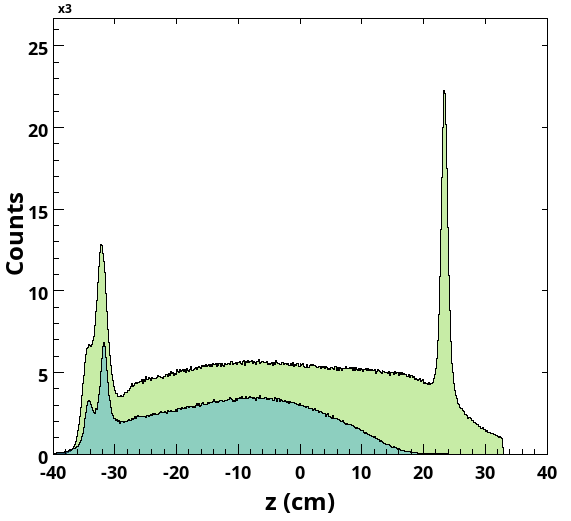
\includegraphics[width=\textwidth]{51vz_012016.png}}
                }
                \scriptsize{\textit{Run \ef{12016}.}}
            \end{figure}
        \end{center}
    \end{column}

    \begin{column}{.35\linewidth}
        \begin{center}
            \begin{figure}[t]
                \centering{
                    \fbox{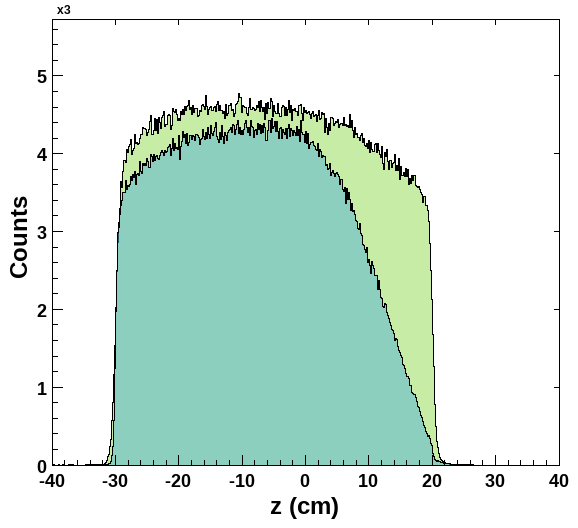
\includegraphics[width=\textwidth]{51vz_999106.png}}
                }
                \scriptsize{\textit{Simulated data.}}
            \end{figure}
        \end{center}
    \end{column}

    \begin{column}{.05\linewidth}\end{column} % Centering column.

    \end{columns}

    \begin{center}
        \scriptsize{\textit{
            \ef{$v_z$} for \textbf{\textcolor[HTML]{c7eca6}{DC (green)}} and \textbf{\textcolor[HTML]{8dcfbf}{FMT (cyan)}} tracks.
        }}
    \end{center}
\end{frame}

% --+ 11.52 ELECTRON VARIABLES +------------------------------------------------
\begin{frame}{Acceptance Correction: $Q^2$ and $\nu$}
    \label{11.52::electron_variables}

    \begin{itemize}
        \item
            A drop in \efe{$Q^2$} acceptance is perceived from \efe{$1$ to $4 \text{ GeV}^2$}.

        \item
            \efe{$\nu$} is within expected parameters.
    \end{itemize}

    \vspace{-12pt}
    \begin{columns}[onlytextwidth,T]

    \begin{column}{.49\linewidth}
        \begin{center}
            \begin{figure}[t]
                \centering{
                    \fbox{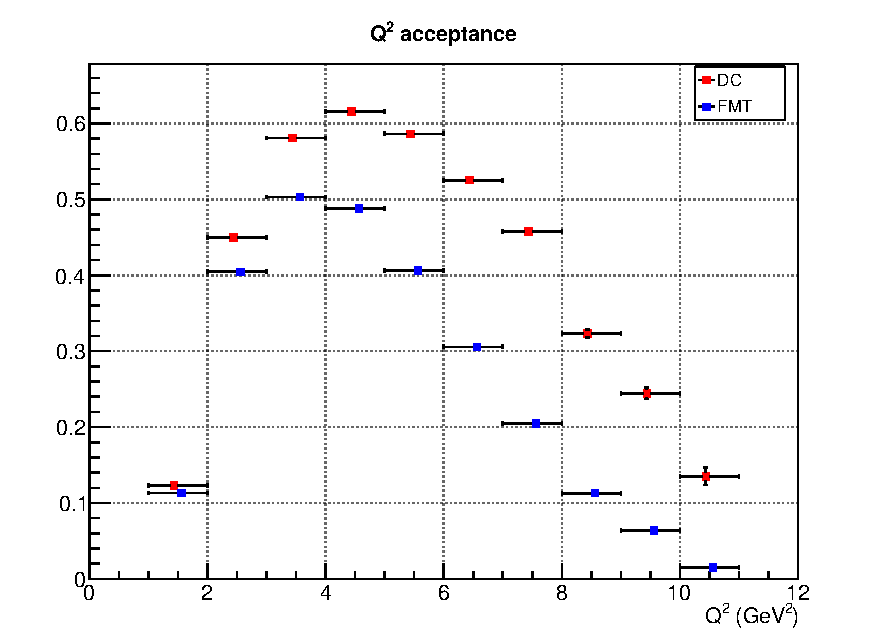
\includegraphics[width=\textwidth]{52q2_acc.pdf}}
                }
                \scriptsize{\textit{
                    \ef{$Q^2$} acceptance for $e^-$.
                    \ef{$\nu$} is integrated.
                }}
            \end{figure}
        \end{center}
    \end{column}

    \begin{column}{.49\linewidth}
        \begin{center}
            \begin{figure}[t]
                \centering{
                    \fbox{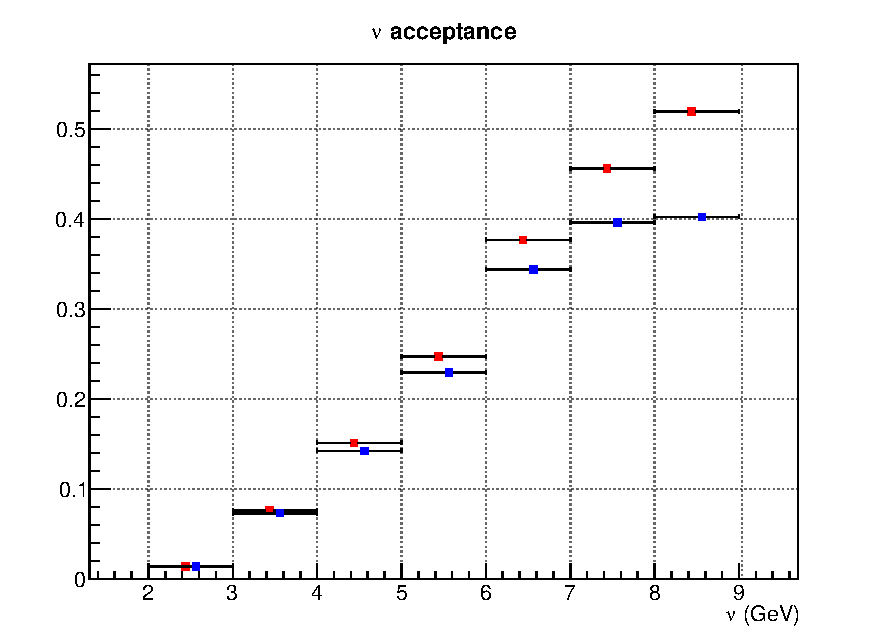
\includegraphics[width=\textwidth]{52nu_acc.pdf}}
                }
                \scriptsize{\textit{
                    \ef{$\nu$} acceptance for $e^-$.
                    \ef{$Q^2$} is integrated.
                }}
            \end{figure}
        \end{center}
    \end{column}

    \end{columns}

    \begin{flushright}
        \tiny{\textit{Bin markers are slightly shifted in $x$ for legibility.}}
        \tiny{\textit{Acceptance error estimation is explained in Slides \textcolor{efd_purple}{\ref{20.11::acceptance_error_estimation}} to \textcolor{efd_purple}{\ref{20.11::acceptance_error_estimation_end}}.}}
    \end{flushright}
\end{frame}

% --+ 11.53 Q2 THETA DEPENDENCE +-----------------------------------------------
\begin{frame}{Acceptance Correction: $Q^2$ $\theta$ dependence}
    \label{11.53::q2_theta_dependence}

    \begin{itemize}
        \item
            \efe{$Q^2$} depends quadratically on the scattered $e^-$ scattering angle \efe{$\theta_C$}.

        \item
            The 6-sector geometry of CLAS12 causes a low efficiency for \efe{$\theta \lsim 0.15$ radians}.

        \item
            This causes the drop in acceptance -- \ef{it is a purely geometric effect}.
    \end{itemize}

    \begin{center}
        \begin{figure}[t]
            \centering{
                \fbox{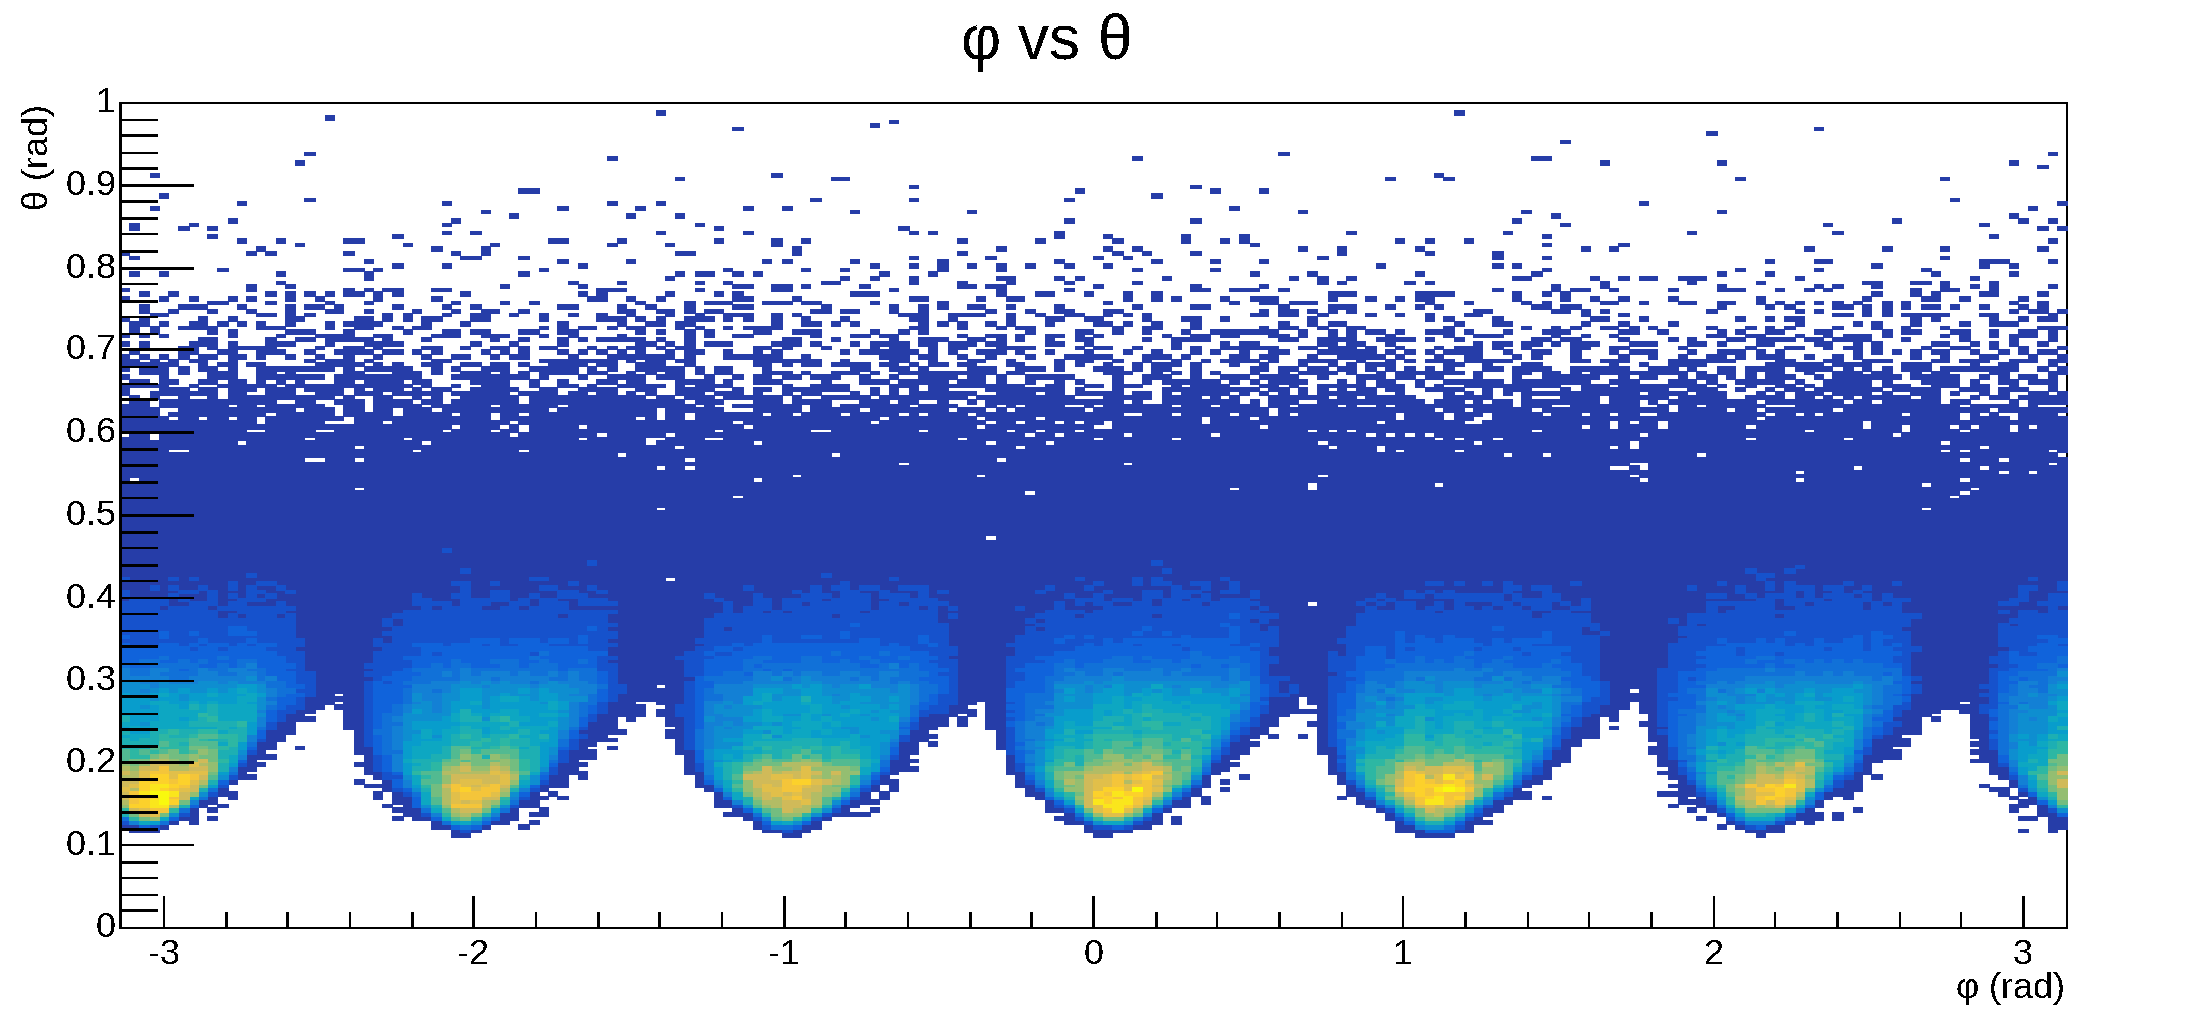
\includegraphics[width=0.8\textwidth]{53phi_theta_neg.pdf}}
            }
        \end{figure}
        \scriptsize{\textit{\ef{$\varphi$} vs. \ef{$\theta$} for negative particles}}
    \end{center}
\end{frame}

% --+ 11.54 ZH +----------------------------------------------------------------
\begin{frame}{Acceptance Correction: $z_h$}
    \label{11.54::zh}

    \begin{itemize}
        % \item
        %     \ef{$z_h$} does not depend on the \ef{$\theta$} of either the hadron or the scattered $e^-$.
        %
        % \vspace{6pt}
        \item
            Since \efe{$z_h$} does not depend on \efe{$\theta$}, its acceptance is intrinsic to CLAS12.

        \vspace{6pt}
        \item
            The larger acceptance of $\pi^+$ is due to the inbending polarity of the solenoid.
    \end{itemize}

    \vspace{-12pt}
    \begin{columns}
        \begin{column}{.49\linewidth}
            \begin{center}
                \begin{figure}[t]
                    \centering{
                        \fbox{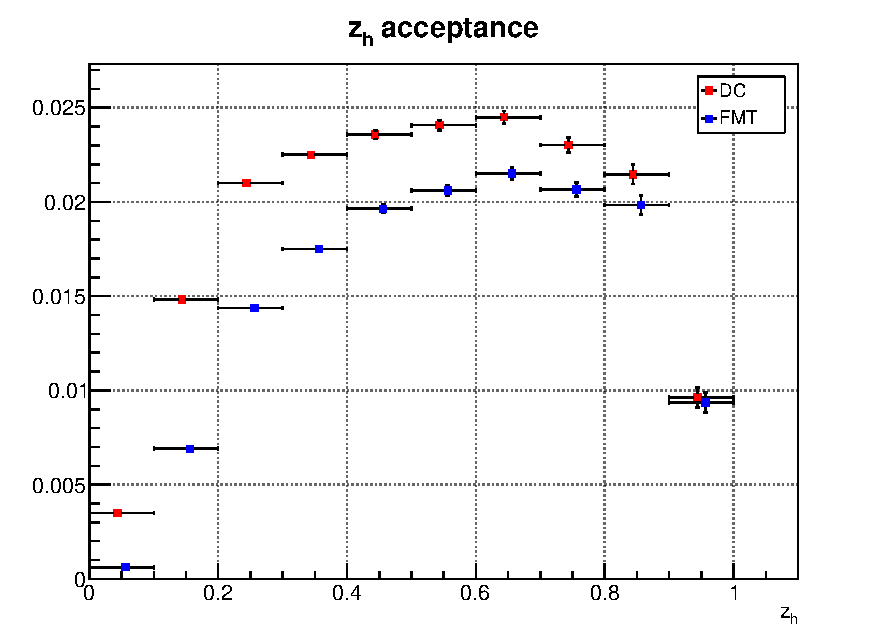
\includegraphics[width=\textwidth]{54zh_acc_-211.pdf}}
                    }
                    \scriptsize{\textit{
                        \ef{$z_h$} acceptance for \ef{$\pi^-$}.
                        Other DIS variables are integrated.
                    }}
                \end{figure}
            \end{center}
        \end{column}

        \begin{column}{.49\linewidth}
            \begin{center}
                \begin{figure}[t]
                    \centering{
                        \fbox{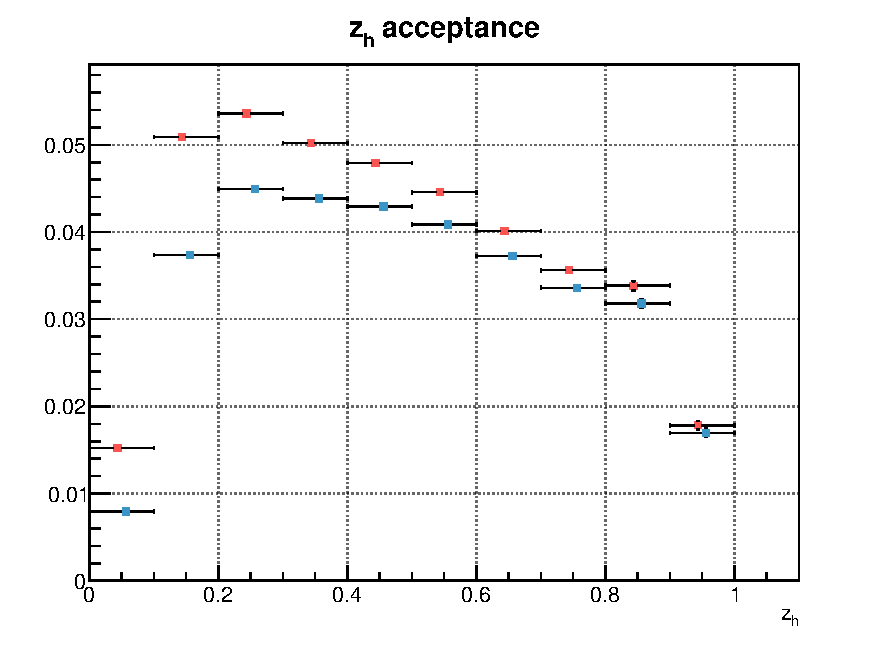
\includegraphics[width=\textwidth]{54zh_acc_211.pdf}}
                    }
                    \scriptsize{\textit{
                        \ef{$z_h$} acceptance for \ef{$\pi^+$}.
                        Other DIS variables are integrated.
                    }}
                \end{figure}
            \end{center}
        \end{column}
    \end{columns}

    \begin{flushright}
        \tiny{\textit{Bin markers are slightly shifted in $x$ for legibility.}}
        \tiny{\textit{Acceptance error estimation is explained in Slides \textcolor{efd_purple}{\ref{20.11::acceptance_error_estimation}} to \textcolor{efd_purple}{\ref{20.11::acceptance_error_estimation_end}}.}}
    \end{flushright}
\end{frame}

% --+ 11.55 PT2 +---------------------------------------------------------------
\begin{frame}{Acceptance Correction: $p_T^2$}
    \label{11.55::pt2}

    \begin{itemize}
        \item
            \ef{$p_T^2$} has a non-trivial dependence on the \ef{$\theta$} of both the $e^-$ and the $\pi^\pm$.

        \vspace{6pt}
        \item
            Very few particles have a \ef{$p_T^2 \gsim 1.4$}, thus the strange values and large errors.
    \end{itemize}

    \vspace{-12pt}
    \begin{columns}
        \begin{column}{.49\linewidth}
            \begin{center}
                \begin{figure}[t]
                    \centering{
                        \fbox{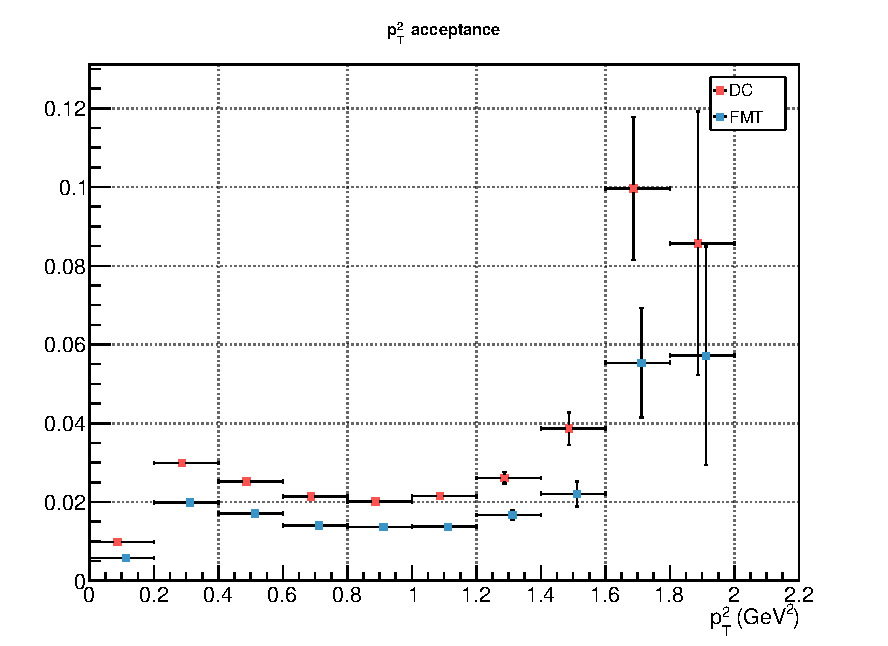
\includegraphics[width=\textwidth]{55pt2_acc_-211.pdf}}
                    }
                    \scriptsize{\textit{
                        \ef{$p_T^2$} acceptance for \ef{$\pi^-$}.
                        Other DIS variables are integrated.
                    }}
                \end{figure}
            \end{center}
        \end{column}

        \begin{column}{.49\linewidth}
            \begin{center}
                \begin{figure}[t]
                    \centering{
                        \fbox{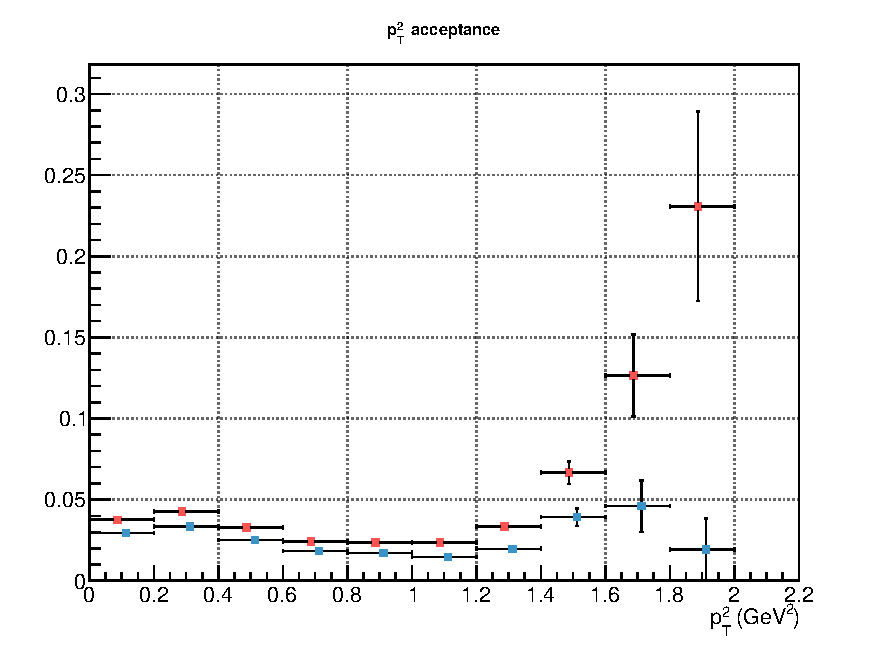
\includegraphics[width=\textwidth]{55pt2_acc_211.pdf}}
                    }
                    \scriptsize{\textit{
                        \ef{$p_T^2$} acceptance for \ef{$\pi^+$}.
                        Other DIS variables are integrated.
                    }}
                \end{figure}
            \end{center}
        \end{column}
    \end{columns}

    \begin{flushright}
        \tiny{\textit{Bin markers are slightly shifted in $x$ for legibility.}}
        \tiny{\textit{Acceptance error estimation is explained in Slides \textcolor{efd_purple}{\ref{20.11::acceptance_error_estimation}} to \textcolor{efd_purple}{\ref{20.11::acceptance_error_estimation_end}}.}}
    \end{flushright}
\end{frame}

% --+ 11.56 PHIPQ +-------------------------------------------------------------
\begin{frame}{Acceptance Correction: $\varphi_{PQ}$}
    \label{11.56::phipq}

    \begin{itemize}
        \item
            \ef{$\varphi_{PQ}$} has a highly non-trivial dependence on the \ef{$\theta$} and \ef{$\varphi$} of the $e^-$ and the $\pi$.

        \vspace{6pt}
        \item
            Distribution shows a similar shape as what is expected from previous analyses.
    \end{itemize}

    \vspace{-12pt}
    \begin{columns}
        \begin{column}{.49\linewidth}
            \begin{center}
                \begin{figure}[t]
                    \centering{
                        \fbox{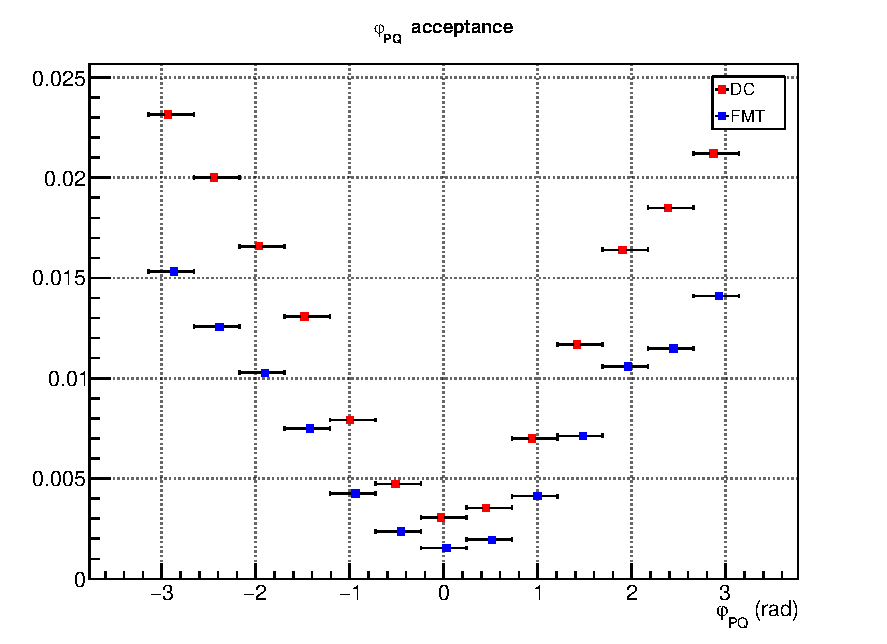
\includegraphics[width=\textwidth]{56phipq_acc_-211.pdf}}
                    }
                    \scriptsize{\textit{
                        \ef{$\varphi_{PQ}$} acceptance for \ef{$\pi^-$}.
                        Other variables are integrated.
                    }}
                \end{figure}
            \end{center}
        \end{column}

        \begin{column}{.49\linewidth}
            \begin{center}
                \begin{figure}[t]
                    \centering{
                        \fbox{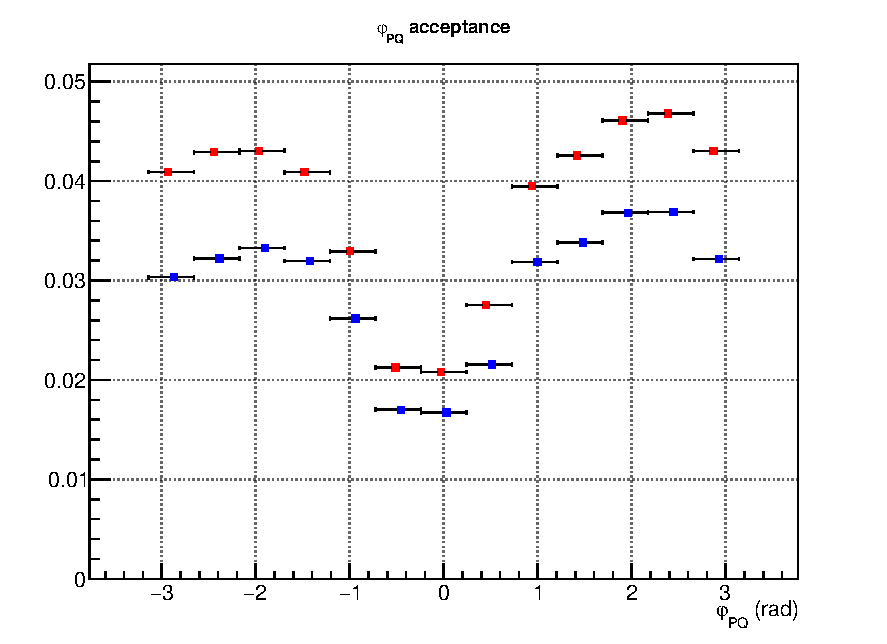
\includegraphics[width=\textwidth]{56phipq_acc_211.pdf}}
                    }
                    \scriptsize{\textit{
                        \ef{$\varphi_{PQ}$} acceptance for \ef{$\pi^+$}.
                        Other variables are integrated.
                    }}
                \end{figure}
            \end{center}
        \end{column}
    \end{columns}

    \begin{flushright}
        \tiny{\textit{Bin markers are slightly shifted in $x$ for legibility.}}
        \tiny{\textit{Acceptance error estimation is explained in Slides \textcolor{efd_purple}{\ref{20.11::acceptance_error_estimation}} to \textcolor{efd_purple}{\ref{20.11::acceptance_error_estimation_end}}.}}
    \end{flushright}
\end{frame}
